\documentclass[9pt]{IEEEtran}

\usepackage[english]{babel}
\usepackage{graphicx}
\usepackage{epstopdf}
\usepackage{fancyhdr}
\usepackage{amsmath}
\usepackage{amsthm}
\usepackage{amssymb}
\usepackage{url}
\usepackage{array}
\usepackage{textcomp}
\usepackage{listings}
\usepackage{hyperref}
\usepackage{xcolor}
\usepackage{colortbl}
\usepackage{float}
\usepackage{gensymb}
\usepackage{longtable}
\usepackage{supertabular}
\usepackage{multicol}
\usepackage[justification=centering]{caption}
\usepackage{amsmath}
\usepackage{caption}
\usepackage{subcaption}
\usepackage[utf8x]{inputenc}

\usepackage[T1]{fontenc}
\usepackage{lmodern}
\usepackage{xcolor}

\input{glyphtounicode}
\pdfgentounicode=1

\graphicspath{{./figures/}}
\DeclareGraphicsExtensions{.pdf,.png,.jpg,.eps}

% correct bad hyphenation here
\hyphenation{op-tical net-works semi-conduc-tor trig-gs}

% ============================================================================================

\title{\vspace{0ex} HW4: Artificial Neural Networks}

\author{Aljaž Konec\vspace{-4.0ex}}

% ============================================================================================

\begin{document}

\maketitle

\section{Introduction}

In this report, we present an implementation of Artificial Neural Networks (ANN) for classification and regression tasks.
Both implementations are compared to the results of the same tasks using the scikit-learn library.
All experiments are performed on the provided housing datasets.


\section{Implementation Details}

Both the classification and regression tasks share a common implementation of the ANN.
Up to the last output layer, both implementations share the same structure where for the activation function we use the sigmoid.
The main differences between the two tasks are:
\begin{itemize}
    \item The number of neurons in the output layer for regression is 1, while for classification it is the number of classes.
    \item The output layer activation function is also different. For the classification task, we use the softmax function, while for the regression task, we use the identity function.
    \item The loss function is different. For the classification task, we use the cross-entropy loss, while for the regression task, we use the mean squared error. Both functions use L2 regularization of the weights only.
\end{itemize}
It turns out, when computing the gradients for loss functions with regars to the weights, both loss functions have the same form of the gradient in the last layer.
Because of this, the implementation of the backpropagation algorithm is the same for both tasks.
For computing the optimal weights, we use Scipy's implementation of the L-BFGS-B optimization algorithm.

\section{Verification of compatibility of gradient and cost functions}
\begin{figure}[!ht]
    \centering
    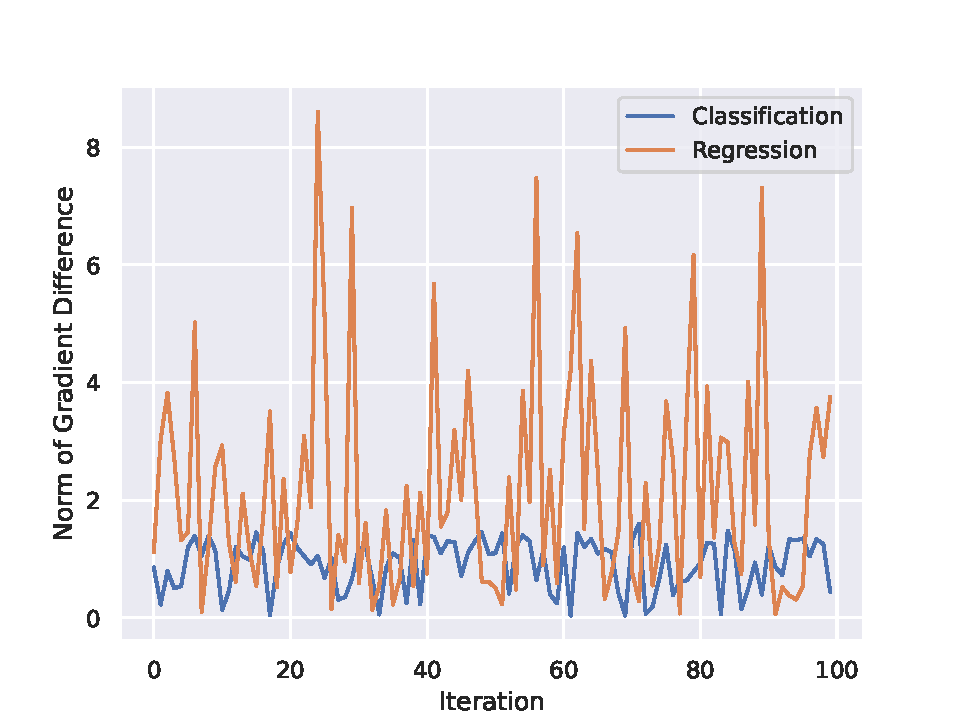
\includegraphics[width=0.5\textwidth]{grad_verification.pdf}
    \caption{Norm of differences between analytical and numerical gradients for different starting weights.}
    \label{fig:grad_verification}
\end{figure}
To verify the compatibility of implemented gradient we compare the gradients to a numerical approximation.
We instantiate the ANN with shape [3, 10, 10, 10, 2] and compute the analytical gradient via the backpropagation algorithm for one backward pass.
We then compute the numerical gradient for weight $w_{ij}^{l}$ between neurons $i$ and $j$ in layer $l$ as:

\begin{equation}
    \frac{\partial C}{\partial w_{ij}^{l}} = \frac{C(x, w_{ij}^{l} + \epsilon) - C(x, w_{ij}^{l} - \epsilon)}{2\epsilon}
\end{equation}    
where $C$ is the cost function, $x$ is the input to the network and $\epsilon = 1e-6$. 
We then compare the analytical gradient to the numerical gradient for all weights in the network by computing norm of the differences:
\begin{equation}
    \text{diff} = || \nabla_{\text{analytical}} - \nabla_{\text{numerical}} ||
\end{equation}


Figure \ref{fig:grad_verification} shows the norm of differences for different starting weights.
To calculate the average difference we generate 100 random starting weights and compute the norm of differences for each starting weight.
Then we used Bootstrap 1000 times to randomly sample 100 norms of differences.
For classification task the norm of diffrences is $0.9140 \pm 0.04475$ and for the regression task it is $2.1775 \pm 0.1848$.
We can see that for classification the norm is smaller and has lower variance than for regression.



\section{Predictions on the Housing Dataset}
In this section we compare our implementation of ANN to multiple other models where we use the provided housing datasets.
All of the data is already in numerical form, so the only preprocessing that we did was to split the data and then normalize it.
We perform an 80-20 split of the data and normalize it using the mean and standard deviation of the training data.

\subsection{Classification Task}
For our ANNClassifier we use hidden layers of size [20, 20] and regularization parameter $\lambda = 0.0001$.
We compare our implementation of ANNClassifier to multiple other logistic regression models:
\begin{itemize}
    \item \textbf{MLPClassifier} - Multi-layer Perceptron classifier from scikit-learn with same hidden layers but $relu$ activation function.
    \item \textbf{MultinomialLogReg\_HW3} - Multinomial Logistic Regression from HW3.
    \item \textbf{LogisticRegression} - Logistic Regression from scikit-learn.
\end{itemize}

Figure \ref{fig:roc} shows the ROC curves for all models.
The best performing models are ANNClassifier and MLPClassifier, with ANNClassifier having a slightly lower AUC score.
Both logistic regression models perform worse at around 0.8 AUC score.
\begin{figure}[H]
    \centering
    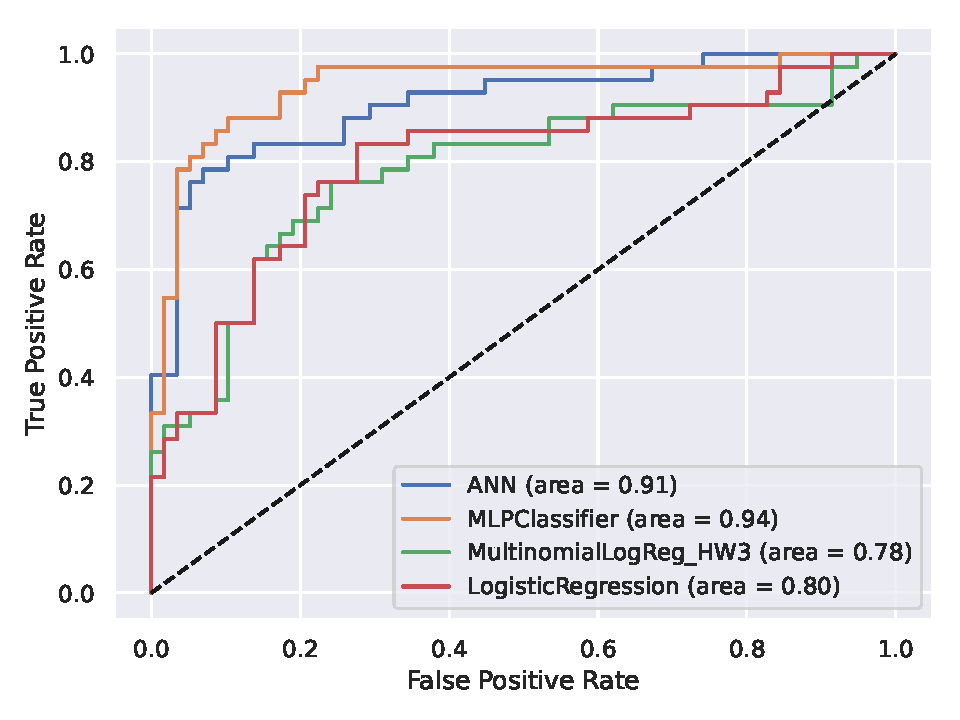
\includegraphics[width=0.488\textwidth]{roc_curve.pdf}
    \caption{ROC curves for all models.}
    \label{fig:roc}
\end{figure}
Table \ref{classification_scores} shows the classification metrics for all models.
The best socring models are again ANN and MLPClassifier, with ANN having a slightly lower precision and recall.
This simple example shows how even a small ANN, with 2 hidden layers, can learn deep representation of the data and outperform basic Logistic Regression models.
\begin{table}[!ht]
    \centering
    \begin{tabular}{lllll}
        \textbf{Model} & \textbf{Precision} & \textbf{Recall} & \textbf{F1} & \textbf{Log-Loss} \\ \hline
        \textbf{ANN} & 0.84 & 0.84 & 0.84 & 0.37 \\ 
        \textbf{MLPClassifier} & 0.88 & 0.88 & 0.88 & 0.37 \\ 
        \textbf{Multinomial-}\\ \textbf{LogReg\_HW3} & 0.76 & 0.6 & 0.47 & 0.66 \\ 
        \textbf{LogisticRegression} & 0.72 & 0.72 & 0.71 & 0.53 \\ 
    \end{tabular}
    \caption{Classification metrics for all tested models.}
    \label{classification_scores}
\end{table}

\subsection{Regression Task}
Similarly to Classification task we build a ANNRegressor model with the hidden layers [20, 20] and compare it to multiple other models:
\begin{itemize}
    \item \textbf{MLPRegressor} - Multi-layer Perceptron regressor from scikit-learn with same hidden layers but $relu$ activation function.
    \item \textbf{LinearRegression} - Linear Regression from scikit-learn.
\end {itemize}





\section{Conclusion}

A sentence or two to conclude the report. Write when the method works well and what its limitations.

\bibliographystyle{IEEEtran}
\bibliography{bibliography}

\end{document}
